\documentclass[12pt]{article}
\usepackage[utf8]{inputenc}
\usepackage{graphicx} % Allows you to insert figures
\usepackage{amsmath} % Allows you to do equations
\usepackage{fancyhdr} % Formats the header
\usepackage{geometry} % Formats the paper size, orientation, and margins
\linespread{1.25} % about 1.5 spacing in Word
\setlength{\parindent}{0pt} % no paragraph indents
\setlength{\parskip}{1em} % paragraphs separated by one line
\usepackage[style=authoryear-ibid,backend=biber,maxbibnames=99,maxcitenames=2,uniquelist=false,isbn=false,url=true,eprint=false,doi=true,giveninits=true,uniquename=init]{biblatex} % Allows you to do citations - does Harvard style and compatible with Zotero
\usepackage{listings}
\usepackage{color} %red, green, blue, yellow, cyan, magenta, black, white
\definecolor{mygreen}{RGB}{28,172,0} % color values Red, Green, Blue
\definecolor{mylilas}{RGB}{170,55,241}
\usepackage{hyperref}
\urlstyle{same} % makes a nicer URL and DOI font 
\AtEveryBibitem{
	\clearfield{urlyear}
	\clearfield{urlmonth}
} % removes access date
\AtEveryBibitem{\clearfield{month}} % removes months in bibliography
\AtEveryCitekey{\clearfield{month}} % removes months in citations
\renewbibmacro{in:}{} % Removes the "In" before journal names

\renewbibmacro*{editorstrg}{%from biblatex.def
	\printtext[editortype]{%
		\iffieldundef{editortype}
		{\ifboolexpr{
				test {\ifnumgreater{\value{editor}}{1}}
				or
				test {\ifandothers{editor}}
			}
			{\bibcpstring{editors}}
			{\bibcpstring{editor}}}
		{\ifbibxstring{\thefield{editortype}}
			{\ifboolexpr{
					test {\ifnumgreater{\value{editor}}{1}}
					or
					test {\ifandothers{editor}}
				}
				{\bibcpstring{\thefield{editortype}s}}%changed
				{\bibcpstring{\thefield{editortype}}}}%changed
			{\thefield{editortype}}}}}

\renewbibmacro*{byeditor+others}{%from biblatex.def
	\ifnameundef{editor}
	{}
	{\printnames[byeditor]{editor}%
		\addspace%added
		\mkbibparens{\usebibmacro{editorstrg}}%added
		\clearname{editor}%
		\newunit}%
	\usebibmacro{byeditorx}%
	\usebibmacro{bytranslator+others}}
% The commands above from lines 20-49 change the way editors are displayed in books
\AtEveryBibitem{%
	\clearlist{language}%
} % removes language from bibliography
\citetrackerfalse 
% Removes ibids (ibidems)
\DeclareNameAlias{sortname}{family-given} % Ensures the names of the authors after the first author are in the correct order in the bibliography
\renewcommand*{\revsdnamepunct}{} % Corrects punctuation for authors with just a first initial
\addbibresource{Example.bib} % Tells LaTeX where the citations are coming from. This is imported from Zotero
\usepackage[format=plain,
font=it]{caption} % Italicizes figure captions
\usepackage[english]{babel}
\usepackage{csquotes}
\renewcommand*{\nameyeardelim}{\addcomma\space} % Adds comma in in-text citations
\renewcommand{\headrulewidth}{0pt}
\geometry{letterpaper, portrait, margin=1in}
\setlength{\headheight}{14.49998pt}

\newcommand\titleofdoc{Reporte práctica cero "Práctica Introducción a Matlab".} %%%%% Put your document title in this argument
\newcommand\GroupName{Laboratorio de Análisis de Sistemas y Señales} %%%%% Put your group name here. If you are the only member of the group, just put your name

\begin{document}
	\lstset{language=Matlab,%
		%basicstyle=\color{red},
		breaklines=true,%
		morekeywords={matlab2tikz},
		keywordstyle=\color{blue},%
		morekeywords=[2]{1}, keywordstyle=[2]{\color{black}},
		identifierstyle=\color{black},%
		stringstyle=\color{mylilas},
		commentstyle=\color{mygreen},%
		showstringspaces=false,%without this there will be a symbol in the places where there is a space
		numbers=left,%
		numberstyle={\tiny \color{black}},% size of the numbers
		numbersep=9pt, % this defines how far the numbers are from the text
		emph=[1]{for,end,break},emphstyle=[1]\color{red}, %some words to emphasise
		%emph=[2]{word1,word2}, emphstyle=[2]{style},    
	}
	\begin{titlepage}
		\begin{center}
			\vspace*{4cm} % Adjust spacings to ensure the title page is generally filled with text
			
			\Huge{\titleofdoc} 
			
			\vspace{0.5cm}
			\LARGE{optional subtitle below}
			
			\vspace{3 cm}
			\Large{\GroupName}
			
			\vspace{0.25cm}
			\large{Miranda Serrano Carlos Alberto, Robles Martínez Héctor}
			
			\vspace{3 cm}
			\Large{Febrero 17, 2022}
			
			\vspace{0.25 cm}
			
			
			\vfill
		\end{center}
	\end{titlepage}
	
	\setcounter{page}{2}
	\pagestyle{fancy}
	\fancyhf{}
	\rhead{\thepage}
	\lhead{\GroupName; \titleofdoc}
	\newpage
	\section{Introducción}
	En esta práctica, aprenderemos a utilizar el lenguaje de programación Matlab, mediante el análisis de funciones senoidales y cosenoidales, de igual manera, analizaremos las partes pares e impares de las señales, aplicándo los conocimientos adquiridos a señales que representen notas musicales específicas. De igual manera, seremos capaces de graficar las señales, tanto en gráficas separadas, gráficas una sobre otra para poder diferenciarlas y gráficas divididas en pequeños subgráficos para poder comparar. Por último, se manejarán archivos de audio reales, para poder obtener señales del mundo real a las que podremos aplicar lo que aprendamos sobre parte par, parte impar, periodicidad y amplitud de una señal.
	\newpage
	\section{Desarrollo de actividades}
	\newpage
	\subsection{Periodo y amplitud de una señal senoidal y otra cosenoidal}
	Considere las siguiente señales:
	\begin{equation}
		x(t) = 2cos(10t+1)-sin(4t-1)
	\end{equation}
	\begin{equation}
		x(t) = [cos(2t- \pi/3)]^2
	\end{equation}
	Determine de ser posible, su periodo y amplitud
	\lstinputlisting{first_6_1.m}
	\begin{figure}[h]
		\centering
		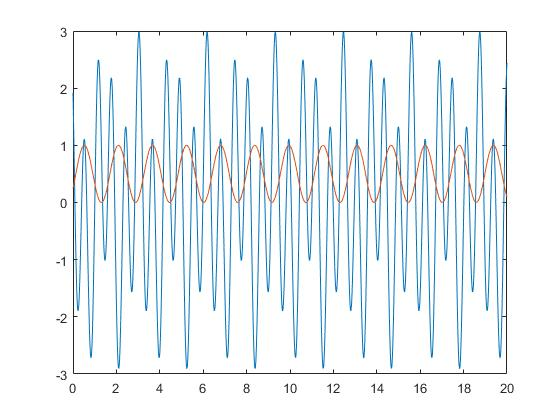
\includegraphics[width=10cm]{6_1.jpg}
	\end{figure}
	\newpage
	\subsection{Periodicidad de la suma de las notas musicales}
	Considere ahora que las notas musicales si, la, sol tienen las siguientes frecuencias.
	\begin{equation}
		f_{si} = 246.942 [Hz]
	\end{equation}
	\begin{equation}
		f_{la} = 220 [Hz]
	\end{equation}
	\begin{equation}
		f_{sol} = 192.998 [Hz]
	\end{equation}
	Donde el sonido se puede definir a través del siguiente modelo matemático:
	\begin{equation}
		x = sin(\omega t + \phi)
	\end{equation}
	Donde \begin{equation*} \omega \end{equation*} es la frecuencia fundamental de cada nota musical. Determine si
	\begin{equation}
		x_1 = x_{la} + x_{si} + x_{sol}
	\end{equation}
	\lstinputlisting{first_6_2.m}
	\begin{figure}[h]
		\centering
		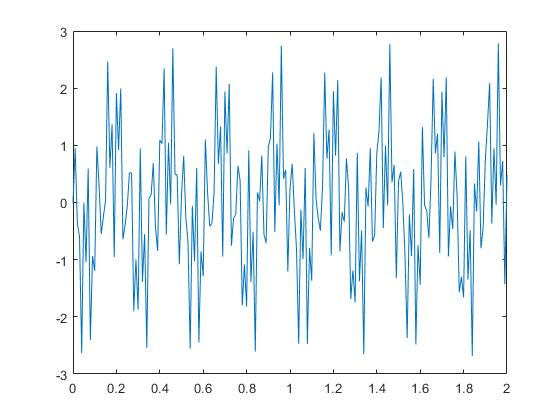
\includegraphics[width=10cm]{6_2.jpg}
	\end{figure}
	\newpage
	\subsection{Parte par e impar}
	De la suma encontrada en el ejercicio anterior, obtenga la parte par e impar de la señal.
	\lstinputlisting{first_6_3.m}
	\begin{figure}[h]
		\centering
		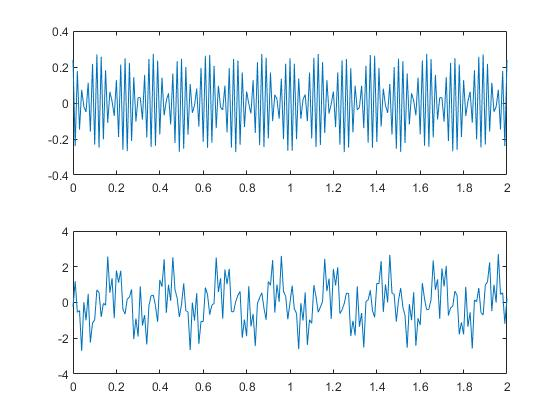
\includegraphics[width=10cm]{6_3.jpg}
	\end{figure}
	\newpage
	\subsection{Archivos de audio}
	Obtenga un archivo de audio y realice las siguientes actividades
	\begin{enumerate}
		\item Obtenga la parte par e impar de la señal
		\item Obtenga la raíz cuadrada y el valor absoluto de la señal de audio ¿cómo se modifica el sonido con cada una de estas operaciones?
		\item Sume dos señales de aurio ¿cómo se modificó la gráfica?
		\item Obtenga las componentes par e impar de la suma anterior
	\end{enumerate}
	Aquí tuvimos problemas para reproducir el audio, pero en clase se escuchó más agudo cuando se obtuvo la raíz cuadrada y muy ruidoso en el valor absoluto.
	\lstinputlisting{first_6_4.m}
	\begin{figure}[h]
		\centering
		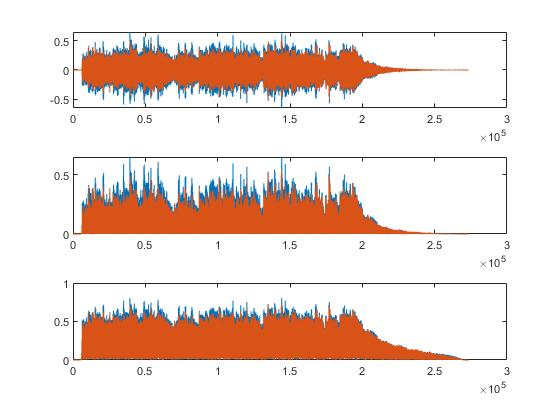
\includegraphics[width=10cm]{6_4_1.jpg}
	\end{figure}
	\begin{figure}[h]
		\centering
		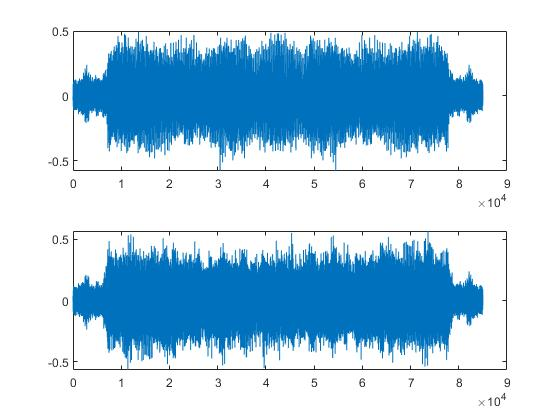
\includegraphics[width=10cm]{6_4_2.jpg}
	\end{figure}
	\newpage
	\section{Análisis de resultados}
	Los resultados de la práctica, concuerdan con lo aprendido en la clase teórica, por lo que podemos confiar en la teoría aplicada a casos reales.
	Es interesante cómo se modifica la señal de audio, y por consecuencia cómo se escucah el audio, al obtener su raíz cuadrada, así como su valor absoluto, es muy diferente al cambio de stereo a mono, donde también combinamos ambos canales de audio en uno solo.
	\newpage
	\section{Conclusiones}
	Podemos recatar muchas cosas aprendidas de la práctica, entre ellas, el uso básico del lenguaje Matlab, así como la observación de los elementos teóricos de la clase con los resultados experimentales obtenidos en esta clase.
	También, podemos ver que no podemos asegurar que una señal es par o impar a simple vista, puesto que se tienen que hacer los desarrollos matemáticos correspondientes para tener la certeza.
	\newpage
	Puede encontrar el código, archivos de audio y demás cosas referentes a la práctica en:
	\url{https://github.com/Hector290601/signals_and_systems/tree/main/practices/first}
\end{document}
